\documentclass[twocolumn,english,pra,aps,superscriptaddress,floatfix]{revtex4-1}

\usepackage{amsthm}
\usepackage{amsmath}
\usepackage{graphicx}
\usepackage{amssymb}
%\usepackage{esint}
\usepackage{bm}
\usepackage{latexsym}

\makeatletter
%%%%%%%%%%%%%%%%%%%%%%%%%%%%%% Textclass specific LaTeX commands.
\@ifundefined{textcolor}{}
{%
 \definecolor{BLACK}{gray}{0}
 \definecolor{WHITE}{gray}{1}
 \definecolor{RED}{rgb}{1,0,0}
 \definecolor{GREEN}{rgb}{0,1,0}
 \definecolor{BLUE}{rgb}{0,0,1}
 \definecolor{CYAN}{cmyk}{1,0,0,0}
 \definecolor{MAGENTA}{cmyk}{0,1,0,0}
 \definecolor{YELLOW}{cmyk}{0,0,1,0}
 }

%%%%%%%%%%%%%%%%%%%%%%%%%%%%%% User specified LaTeX commands.
%\numberwithin{equation}{section}

\makeatother

\usepackage{babel}

\begin{document}



\author{N. Miladinovic}
\affiliation{Department of Physics and Astronomy, McMaster University, 1280 Main
St.\ W., Hamilton, ON, L8S 4M1, Canada} 
\author{D.\ H.\ J.\ O'Dell}
\affiliation{Department of Physics and Astronomy, McMaster University, 1280 Main
St.\ W., Hamilton, ON, L8S 4M1, Canada}

\title{The optical He-McKellar-Wilkens phase and its connection to the Abraham-Minkowski controversy}
\date{\today}

\begin{abstract}
\label{sec:abstract}
Here we are examining a Kapitza-Dirac interferometer similar to that described in the Ketterle paper, with the exception of including a plane wave laser which adds an additional HMW phase.  We then go on to look at a triple Brag grating Mach-Zehnder interferomter. Finally we look at the Hinds-Barnett pulsed result and make sure we understand the result from a quantum perspective by working out the expectation value of the momentum inside of the pulse.
\end{abstract}
%\pacs{42.50.Ex, 42.50.Pq, 42.60.Da, 42.82.Et, 03.67.Lx}

\maketitle

%*********************************************************
\section{Kapitza-Dirac Interferometer}
\label{sec:kaptiza}
%*********************************************************

Here we consider a Bose Einstein condensate placed in a uniform travelling wave laser.  We assume initially the BEC is magnetically trapped and confined in some region while a plane wave laser is acting on it.  The trap is then turned off and a standing pulse is applied to the BEC.  The reason we want the laser on before the standing pulse is because we want to only observe the HMW phase shift without having to deal with the classical forces associated with entering a laser.
After the first pulse, a fraction of the atoms are scattered into the $\pm 2n_r\hbar k$ momentum states, while a fraction remains in a ground state. Here $k$ is the recoil momentum and $n_r$ is the refractive index of the BEC.  (In the Ketterle experiment \cite{ketterle}, their parameters gave a refractive index of $n_r=1.05$.) After a $6$ms delay, a second standing pulse is applied which kicks the $\pm 2n_r\hbar k$ group back into the ground state and produces an interference pattern which may be observed. 
%***************************figure**********************
\begin{figure}
\includegraphics[width=1\columnwidth]{KapitzaDirac.pdf}
\caption{In (A) the initial configuration is a Rubidium BEC in a harmonic trap illuminated by a laser. (B) The trap is then dropped and the BEC is pulsed with a standing beam which scatters a fraction of the atoms into $\pm \hbar k$ states.  (C) After a delay of $3$ms, a second standing pulse will scatter another group out of the ground group which interfere with the first scattered group.} 
\label{fig:kapitz}
\end{figure}
%*********************************************************

The dipole potential created by a standing wave pulse is given by
\begin{equation}
\mathrm{U(\mathbf{x},t)=\frac{\hbar \Omega_R^2}{\Delta}f^2(t)\sin{(n_rk\mathbf{x})}}
\end{equation}
Where $\Omega_R$ is the Rabi frequency and $\Delta$ is the detuning away from the atomic transition frequency.  Here we have assumed $\Delta^2 \gg \Gamma/4$, where $\Gamma$ is the spontaneous decay rate. The function $f$ can be any function, but we will assume it is a simple step function resulting in a square wave pulse.
In the Raman-Nath approximation, the wave function immediately following a Kapitza-Dirac pulse is \cite{meystre,ketterle}
\begin{equation}
\left|\psi\right>=\left|\psi_0\right>e^{\frac{-i}{\hbar}\int dt'\,U(x,t')}=\left|\psi_0\right>e^{\frac{-i}{2\Delta}\Omega_R^2\tau}e^{\frac{i}{2\Delta}\Omega_R^2\tau\cos{(2n_rkx)}}
\end{equation}
Here we have defined $\tau=\int dt' f^2(t')$ which for a square wave pulse is simply the interaction time $\tau=t_{\mathrm{int}}$.  Note that for Kapitza-Dirac standing wave pulses we are assuming short interaction times relative to the recoil frequency (i.e.\, $t\ll 1/\omega_{\mathrm{rec}}$).  During the pulse we assume the atomic motion is negligible.   Making use of the identity 
\begin{equation}
e^{iA\cos{(B)}}=\sum\limits_{m=-\infty}^{\infty}i^mJ_m(A)e^{imB}
\end{equation}
we rewrite the wave function in terms of Bessel functions of the first kind
\begin{eqnarray}
\left|\psi\right>&=&\left|\psi_0\right>e^{\frac{-i\Omega_R^2\tau}{2\Delta}}\sum\limits_{m=-\infty}^{\infty}i^mJ_m\left(\frac{\Omega_R^2\tau}{2\Delta}\right)e^{i2mn_rkx} \nonumber \\
&=&e^{\frac{-i\Omega_R^2\tau}{2\Delta}}\sum\limits_{m=-\infty}^{\infty}i^mJ_m\left(\frac{\Omega_R^2\tau}{2\Delta}\right)\left|2mn_r\hbar k\right>
\end{eqnarray}
The Hamiltonian after the first pulse has acted is given by
\begin{eqnarray}
\hat{H}&=&\mathrm{\frac{\left(\hat{P}+\mathbf{d}\times\mathbf{B}\right)^2}{2m}-\frac{1}{2}\alpha E^2}\nonumber \\
&=&\mathrm{\frac{\hat{P}^2+2\mathbf{d}\times\mathbf{B}\hat{P}+\left(\mathbf{d}\times\mathbf{B}\right)^2}{2m}-\frac{1}{2}\alpha E^2}\nonumber \\
\end{eqnarray}

This is true since the R\"{o}ntgen term $\mathbf{d}\times\mathbf{B}$ is constant in this setup.  Since plane waves are eigenstates of the Hamiltonian, the eigenvalue of the term $\mathrm{\hat{P}}$ is
\begin{equation}
\mathrm{\hat{P} e^{\pm i2n_rkx}=\pm2n_r\hbar k e^{\pm i2n_rkx}}
\end{equation}
and therefore
\begin{equation}
\mathrm{\hat{H} e^{\pm i2n_rkx}=\left[\frac{\left(\pm 2n_r\hbar k+\mathbf{d}\times\mathbf{B}\right)^2}{2m}-\frac{1}{2}\alpha E^2\right]e^{\pm i2n_rkx}}
\end{equation}
We will drop the phase factor appearing in front of the summation in what follows. From here we can determine the state of the wave function $\psi$ at any time $t$ after the pulse.  In the position space representation this is found to be 
\begin{eqnarray}
&&\mathrm{\psi(x,t+\tau)=e^{\frac{-i\hat{H}t}{\hbar}}\psi(0)} \nonumber \\
&&=\mathrm{J_0\left(\frac{\Omega_R^2\tau}{2\Delta}\right)e^{\frac{-i}{\hbar}\left[\frac{\left(\mathbf{d}\times\mathbf{B}\right)^2}{2m}-\frac{1}{2}\alpha E^2\right]t}\left|0n_r\hbar k\right>} \nonumber \\
&+&\mathrm{iJ_1\left(\frac{\Omega_R^2\tau}{2\Delta}\right)\left(e^{i2n_rkx-\frac{it}{\hbar}\left[\frac{\left( 2n_r\hbar k+\mathbf{d}\times\mathbf{B}\right)^2}{2m}-\frac{1}{2}\alpha E^2\right]}\right)\left|2n_r\hbar k\right>} \nonumber \\
&+&\mathrm{iJ_1\left(\frac{\Omega_R^2\tau}{2\Delta}\right)\left(e^{-i2n_rkx-\frac{it}{\hbar}\left[\frac{\left(-2n_r\hbar k+\mathbf{d}\times\mathbf{B}\right)^2}{2m}-\frac{1}{2}\alpha E^2\right]}\right)\left|-2n_r\hbar k\right>} \nonumber \\
&&=\mathrm{e^{\frac{-it}{\hbar}\left(\frac{\left(\mathbf{d}\times\mathbf{B}\right)^2}{2m}-\frac{1}{2}\alpha E^2\right)}\bigg(J_0\left(\frac{\Omega_R^2\tau}{2\Delta}\right)\left|0n_r\hbar k\right>}\nonumber \\
&&+\mathrm{iJ_1\left(\frac{\Omega_R^2\tau}{2\Delta}\right)e^{i\left(2n_rkx-\frac{4\hbar^2n_r^2k^2t}{2m\hbar}-2n_rk\frac{\mathbf{d}\times\mathbf{B}}{m}t\right)}\left|2n_r\hbar k\right>}\nonumber \\
&&+\mathrm{iJ_1\left(\frac{\Omega_R^2\tau}{2\Delta}\right)e^{i\left(-2n_rkx-\frac{4\hbar^2n_r^2k^2t}{2m\hbar}+2n_rk\frac{\mathbf{d}\times\mathbf{B}}{m}t\right)}\left|-2n_r\hbar k\right>\bigg)}
\end{eqnarray}
Here we have made use of the identity $J_{-m}(\theta)=(-1)^mJ_{m}(\theta)$.  


We next apply another standing wave pulse to this wave function. We are interested in finding the probability of finding the atoms in the ground state $\left|0n_r\hbar k\right>$ after this second pulse, so we are only interested in the $\left|0n_r\hbar k\right>$ terms.
\begin{eqnarray}
&&\mathrm{\psi(x,t+2\tau)=\mathrm{e^{\frac{-it}{\hbar}\left(\frac{\left(\mathbf{d}\times\mathbf{B}\right)^2}{2m}-\frac{1}{2}\alpha E^2\right)}\bigg(J_0^2\left(\frac{\Omega_R^2\tau}{2\Delta}\right)\left|0n_r\hbar k\right>}}\nonumber \\
&&-\mathrm{J_1^2\left(\frac{\Omega_R^2\tau}{2\Delta}\right)e^{i\left(2n_rkx-\frac{4\hbar^2n_r^2k^2t}{2m\hbar}-2n_rk\frac{\mathbf{d}\times\mathbf{B}}{m}t\right)}\left|0n_r\hbar k\right>}\nonumber \\
&&-\mathrm{J_1^2\left(\frac{\Omega_R^2\tau}{2\Delta}\right)e^{i\left(-2n_rkx-\frac{4\hbar^2n_r^2k^2t}{2m\hbar}+2n_rk\frac{\mathbf{d}\times\mathbf{B}}{m}t\right)}\left|0n_r\hbar k\right>\bigg)}
\end{eqnarray}

The probability $p_0$ of finding the atoms in the ground state $\left|0n_r\hbar k\right>$ is

\begin{eqnarray}
\mathrm{p_0=|\left<\psi(x,t+2\tau)|0n_r\hbar k\right>|^2=J_0^4\left(\frac{\Omega_R^2\tau}{2\Delta}\right)}\nonumber \\
\mathrm{-4J_0^2\left(\frac{\Omega_R^2\tau}{2\Delta}\right)J_1^2\left(\frac{\Omega_R^2\tau}{2\Delta}\right)\cos{\left(\frac{4\hbar^2n_r^2k^2t}{2m\hbar}\right)}}\nonumber \\
\mathrm{\times cos{\left(2n_rkx-2\frac{\mathbf{d}\times\mathbf{B}}{m}n_rkt\right)}} \nonumber \\
\mathrm{+4J_1^4\left(\frac{\Omega_R^2\tau}{2\Delta}\right)\cos^2{\left(2n_rkx-2\frac{\mathbf{d}\times\mathbf{B}}{m}n_rkt\right)}}
\label{prob1}
\end{eqnarray}
The third term can be dropped as $J_0^2J_1^2\gg J_1^4$.  

Thus far we have neglected the impact that the doppler shifted dipole term would have on our ability to see the HMW phase.  Without the doppler shift, the dipole term $\frac{1}{2}\alpha E^2$ does not affect the probability since it contributes equally to all momentum states.  The doppler shift presents itself through the detuning 
\begin{equation}
\mathrm{\Delta_{\pm}=\Delta\left(1\pm \frac{\omega_{L}}{\Delta}\frac{v}{c}\right)}
\end{equation}
The doppler shifted dipole term is
\begin{equation}
\mathrm{\frac{1}{2}\alpha\left(1\mp \frac{\omega_{L}}{\Delta}\frac{v}{c}\right)E^2}
\end{equation}
If we include this term, the probability amplitude becomes
\begin{eqnarray}
&&\mathrm{p_0=|\left<\psi(x,t+2\tau)|0n_r\hbar k\right>|^2=J_0^4}\nonumber \\
&&\mathrm{-4J_0^2J_1^2\cos{\left(\frac{4\hbar^2n_r^2k^2t}{2m\hbar}\right)}\cos{\left(2n_rkx-2\frac{\mathbf{d}\times\mathbf{B}}{m}n_rkt+\frac{1}{2}\alpha E^2\frac{\omega_L}{\hbar \Delta}\frac{v}{c}t\right)}} \nonumber \\
&&\mathrm{+4J_1^4\cos^2{\left(2n_rkx-2\frac{\mathbf{d}\times\mathbf{B}}{m}n_rkt+\frac{1}{2}\alpha E^2\frac{\omega_L}{\hbar \Delta}\frac{v}{c}t\right)}} \nonumber \\
&&=J_0^4-\mathrm{-4J_0^2J_1^2\cos{\left(\frac{4\hbar^2n_r^2k^2t}{2m\hbar}\right)}\cos{\left(2n_rkx-2\alpha E^2\frac{n_rkt}{mc}\left(1-\frac{\omega_L}{2\Delta}\right)\right)}} \nonumber \\
\label{prob2}
\end{eqnarray}

Where in the last line we have dropped the higher order term. Comparing  Eq.\ (\ref{prob1}) with  Eq.\ (\ref{prob2}) we see that the dipole effect must be dealt with by running the traveling wave laser in both directions in order to isolate the contribution from the HMW phase.
\vspace{5mm}
 
The difficulty in realizing this effect experimentally hangs in the ability to maximize the contribution due to the HMW phase, while suppressing spontaneous emission. The HMW phase is incredibly small and requires a large intensity to become visible. The danger in pushing the intensity high is that spontaneous emission begins to creep into the picture. The Rayleigh scattering rate $\gamma_{R}$
is given by
\begin{equation}
\mathrm{\gamma_{R}=\frac{I\alpha ^2 k^3}{6 \pi\epsilon_{0}^2 c\hbar}}
\label{scatter}
\end{equation}
Where $I=\frac{1}{2}c\epsilon_0 E^2$ is the intensity of the beam. The goal is then to find a regime in which we may observe the HMW phase without spontaneous emission. We can get a sense of the required magnitude of the HMW to obtain an observable effect by considering the time-energy uncertainty relation $\Delta E \Delta t>\hbar/2$.  This uncertainty relation tells us that during a 1ms sampling time, we require an angular frequency shift of $\Delta \omega>500\,\mathrm{Hz}$ which we round to 1kHz. Setting this equal to the HMW frequency $2\frac{\mathbf{d}\times\mathbf{B}}{m}n_rkt$ we find that $\alpha I>4\times 10^{-25}$. Here $I$ is the intensity and $\alpha$ is the polarizability. Substituting this into Eq.\ (\ref{scatter}) gives us $\alpha<6\times10^-40$.  Such a polarizability may be acheived by using a wave length $\lambda=1064$nm, which yields a D1 ground state polarizability for Lithium of $\alpha =5.1\times 10^{-40} \,\mathrm{F\cdot m^2}$, with a detuning of $\Delta=6\times10^{14}$ Hz. This follows from $\alpha(\omega)=\alpha\frac{\omega_0^2}{\omega^2-\omega_0^2}$ \cite{steck}, where $\omega_0$ is the D1 resonant frequency, and $\alpha$ is the dc polarizability for Lithium.  As a result of using such a large detuning, we require a laser intensity of $\mathrm{I=10^{11}\,W/cm^2}$. Using this we find $\frac{1}{2}\alpha E^2=1.9\times 10^{-22}$ J. In free space, such a high power output would be difficult to achieve, but by placing the atom in a ring cavity (Figure \ref{fig:ringcavity}) we can enhance the intensity by a factor of $2\mathcal{F}/\pi$ \cite{spectroscopy}, where $\mathcal{F}$ is the finesse of the cavity system.  The cavity finesse required will of course depend on the intensity of the pump laser.
A caveat of placing the atom in a cavity system is that a back action of the atom on the intra-cavity field can alter the cavity modes. Collective atom recoil lasing (CARL) instabilities can arise in such a system \cite{courteille}.  CARL labels any type of behavior in a atom-cavity system in which feedback from the atom on the cavity modes cause atomic density modulation and/or growth of optical fields.  As an example of a potential pitfall to placing the atom inside a cavity is the possibility that the atom will radiate into the oppositely traveling mode of the ring cavity and hence setup a lattice.  Such an effect would obviously be undesirable as the dipole force generated by an optical lattice would add an extra layer of complication to disentangling the HMW phase from other effects.  For a single atom massively detuned from the cavity mode, it turns out that even for such high intensities such as those required to see the HMW phase, the CARL threshold is not reached \cite{hemmerich} and the back action effects may safely be ignored.  
%***************************figure**********************
\begin{figure}
\includegraphics[width=1\columnwidth]{RingCavity.pdf}
\caption{A schematic for the high finesse ring cavity setup used to enhance the intensity of the traveling wave. The cavity mode must be massively detuned from the atomic transition in order to suppress spontaneous emission $\gamma$. } 
\label{fig:ringcavity}
\end{figure}
%*********************************************************

Using a Kaptiza-Dirac pulse of wavelength $\lambda=780\,\mathrm{nm}$ the value of the recoil frequency term is $\frac{4\hbar^2n_r^2k^2t}{2m\hbar}=1.1\times 10^6\, t$, while $n_r\hbar kx$ is approximately twice the size of the recoil term. The R\"{o}ntgen term which is responsible for the HMW phase is  $2\frac{\mathbf{d}\times\mathbf{B}}{m}n_rk\,t=1.8\times10^3\,t$.  This gives  a noticeable shift in the probability amplitude Eq.\ (\ref{prob1}).
In figure \ref{fig:ft2hk} we plot the probability of finding the atom in the ground state with and without the HMW phase using these values. The red line shows the probability to find the atoms in the ground state without the HMW phase, while the solid blue lines include the HMW phase.
%***************************figure**********************
\begin{figure}
\includegraphics[width=1\columnwidth]{Probability2hk.pdf}
\caption{A plot of the probability of finding the atoms in the ground state $\mathrm{p_0=|\left<\psi(x,t+2\tau)|0n\hbar k\right>|^2}$. The red line show the probability of finding the atoms in the ground state without the HMW phase, while the blue line include the HMW phase.} 
\label{fig:prob}
\end{figure}
%*********************************************************

The spontaneous emission rate at $\mathrm{I=10^{11}\,W/cm^2}$ is $\gamma_{R}\approx \mathrm{10^{-3}\,s}$ which is long enough to measure the HMW phase without worrying about the decohering effects of spontaneous emission.

A possible enhancing technique which may also be implemented to increase the size of the R\"{o}ntgen term is to consider large momentum transfer beamsplitters (LMT). Thus far we have only considered recoil momentum kicks of the form $2n_r\hbar k$. However, it is possible to use large momentum transfers on the order of $10 n_r\hbar k-100 n_r\hbar k$ \cite{kasevich}.  Using such an LMT, we would could significantly increase the effects of the HMW phase..  In Figures \ref{fig:ft2hk} and \ref{fig:ft10hk} we plot the time-discrete fourier transform of Eq.\ (\ref{prob1}) using a $2n_r\hbar k$ and a $10n_r\hbar k$ momentum transfer respectively.
%***************************figure**********************
\begin{figure}
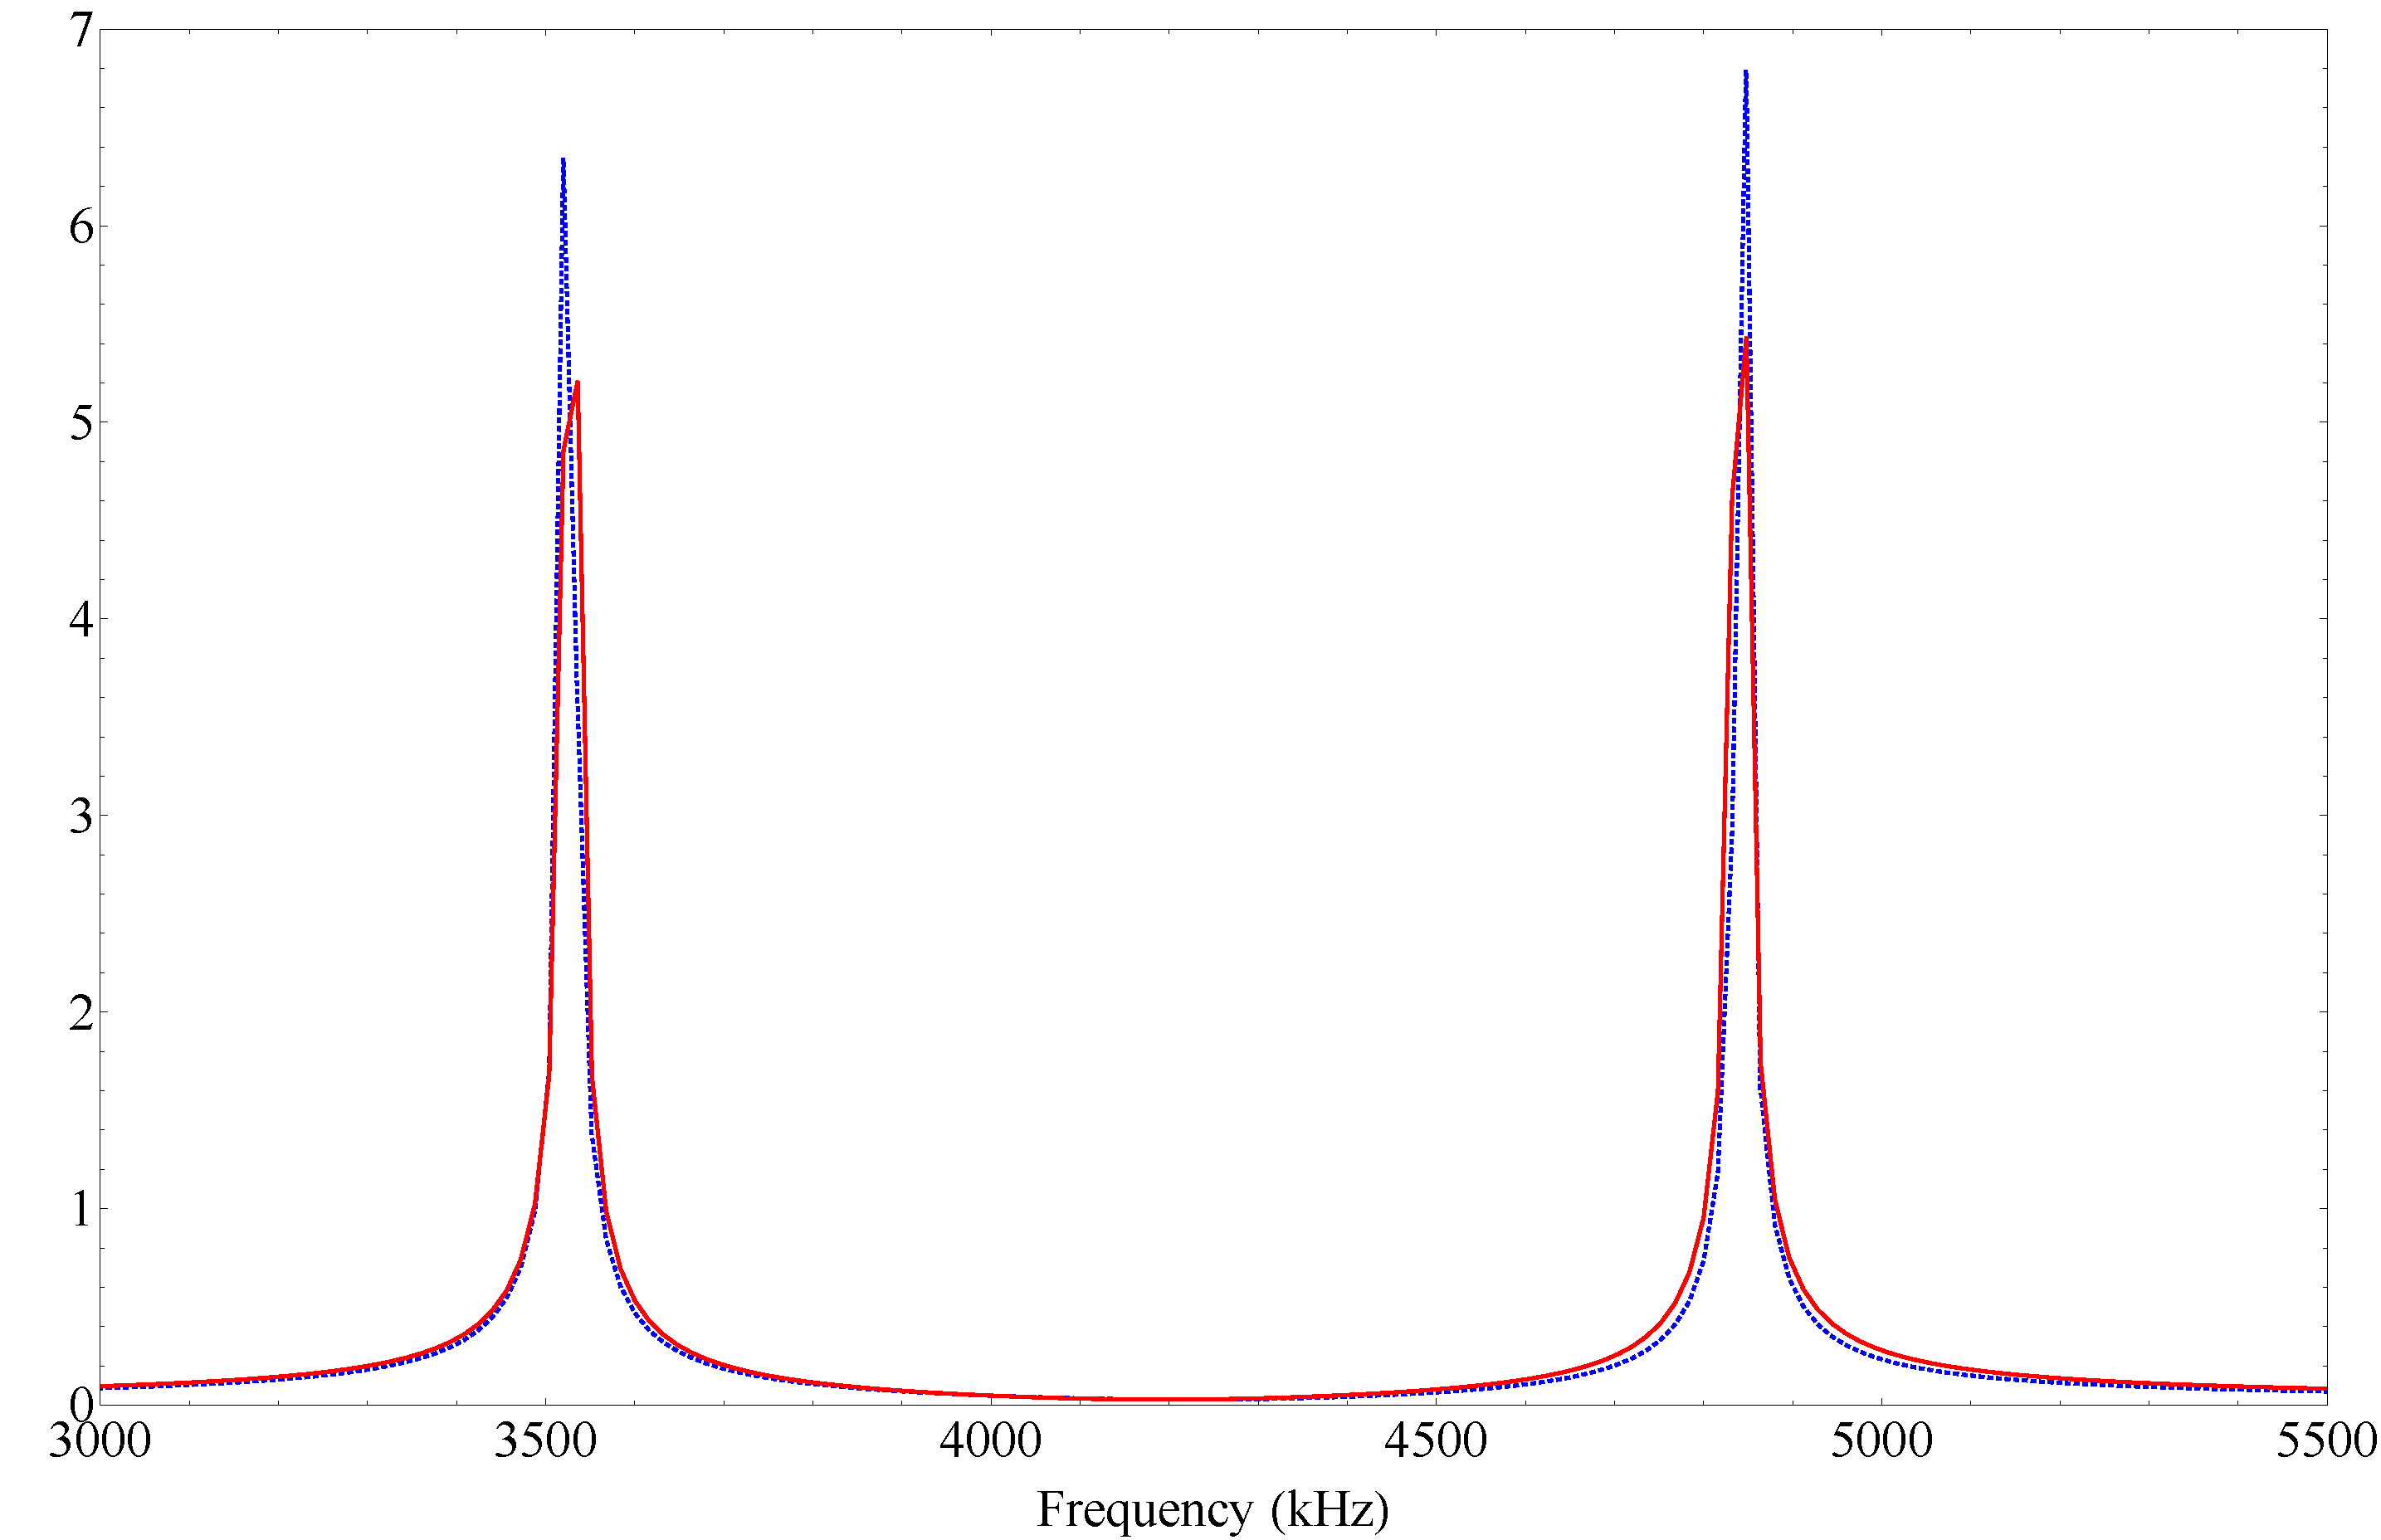
\includegraphics[width=1\columnwidth]{FT2hk.pdf}
\caption{The time-discrete fourier transform of Eq.\ (\ref{prob1}) using 1ms of sampling with a 1$\mu$s sample rate. The dotted blue line shows the fourier transform without the HMW phase, while the red line include the HMW phase. The effect of the HMW on the fourier transform is most apparent in the magnitude change, while the frequency shift is difficult to see.  To make the signature more striking, we can increase the momentum transfer from $2\hbar k$ used in this simulation, to a $10\hbar k$ kick used in figure \ref{fig:ft10hk}.} 
\label{fig:ft2hk}
\end{figure}
%*********************************************************

%***************************figure**********************
\begin{figure}
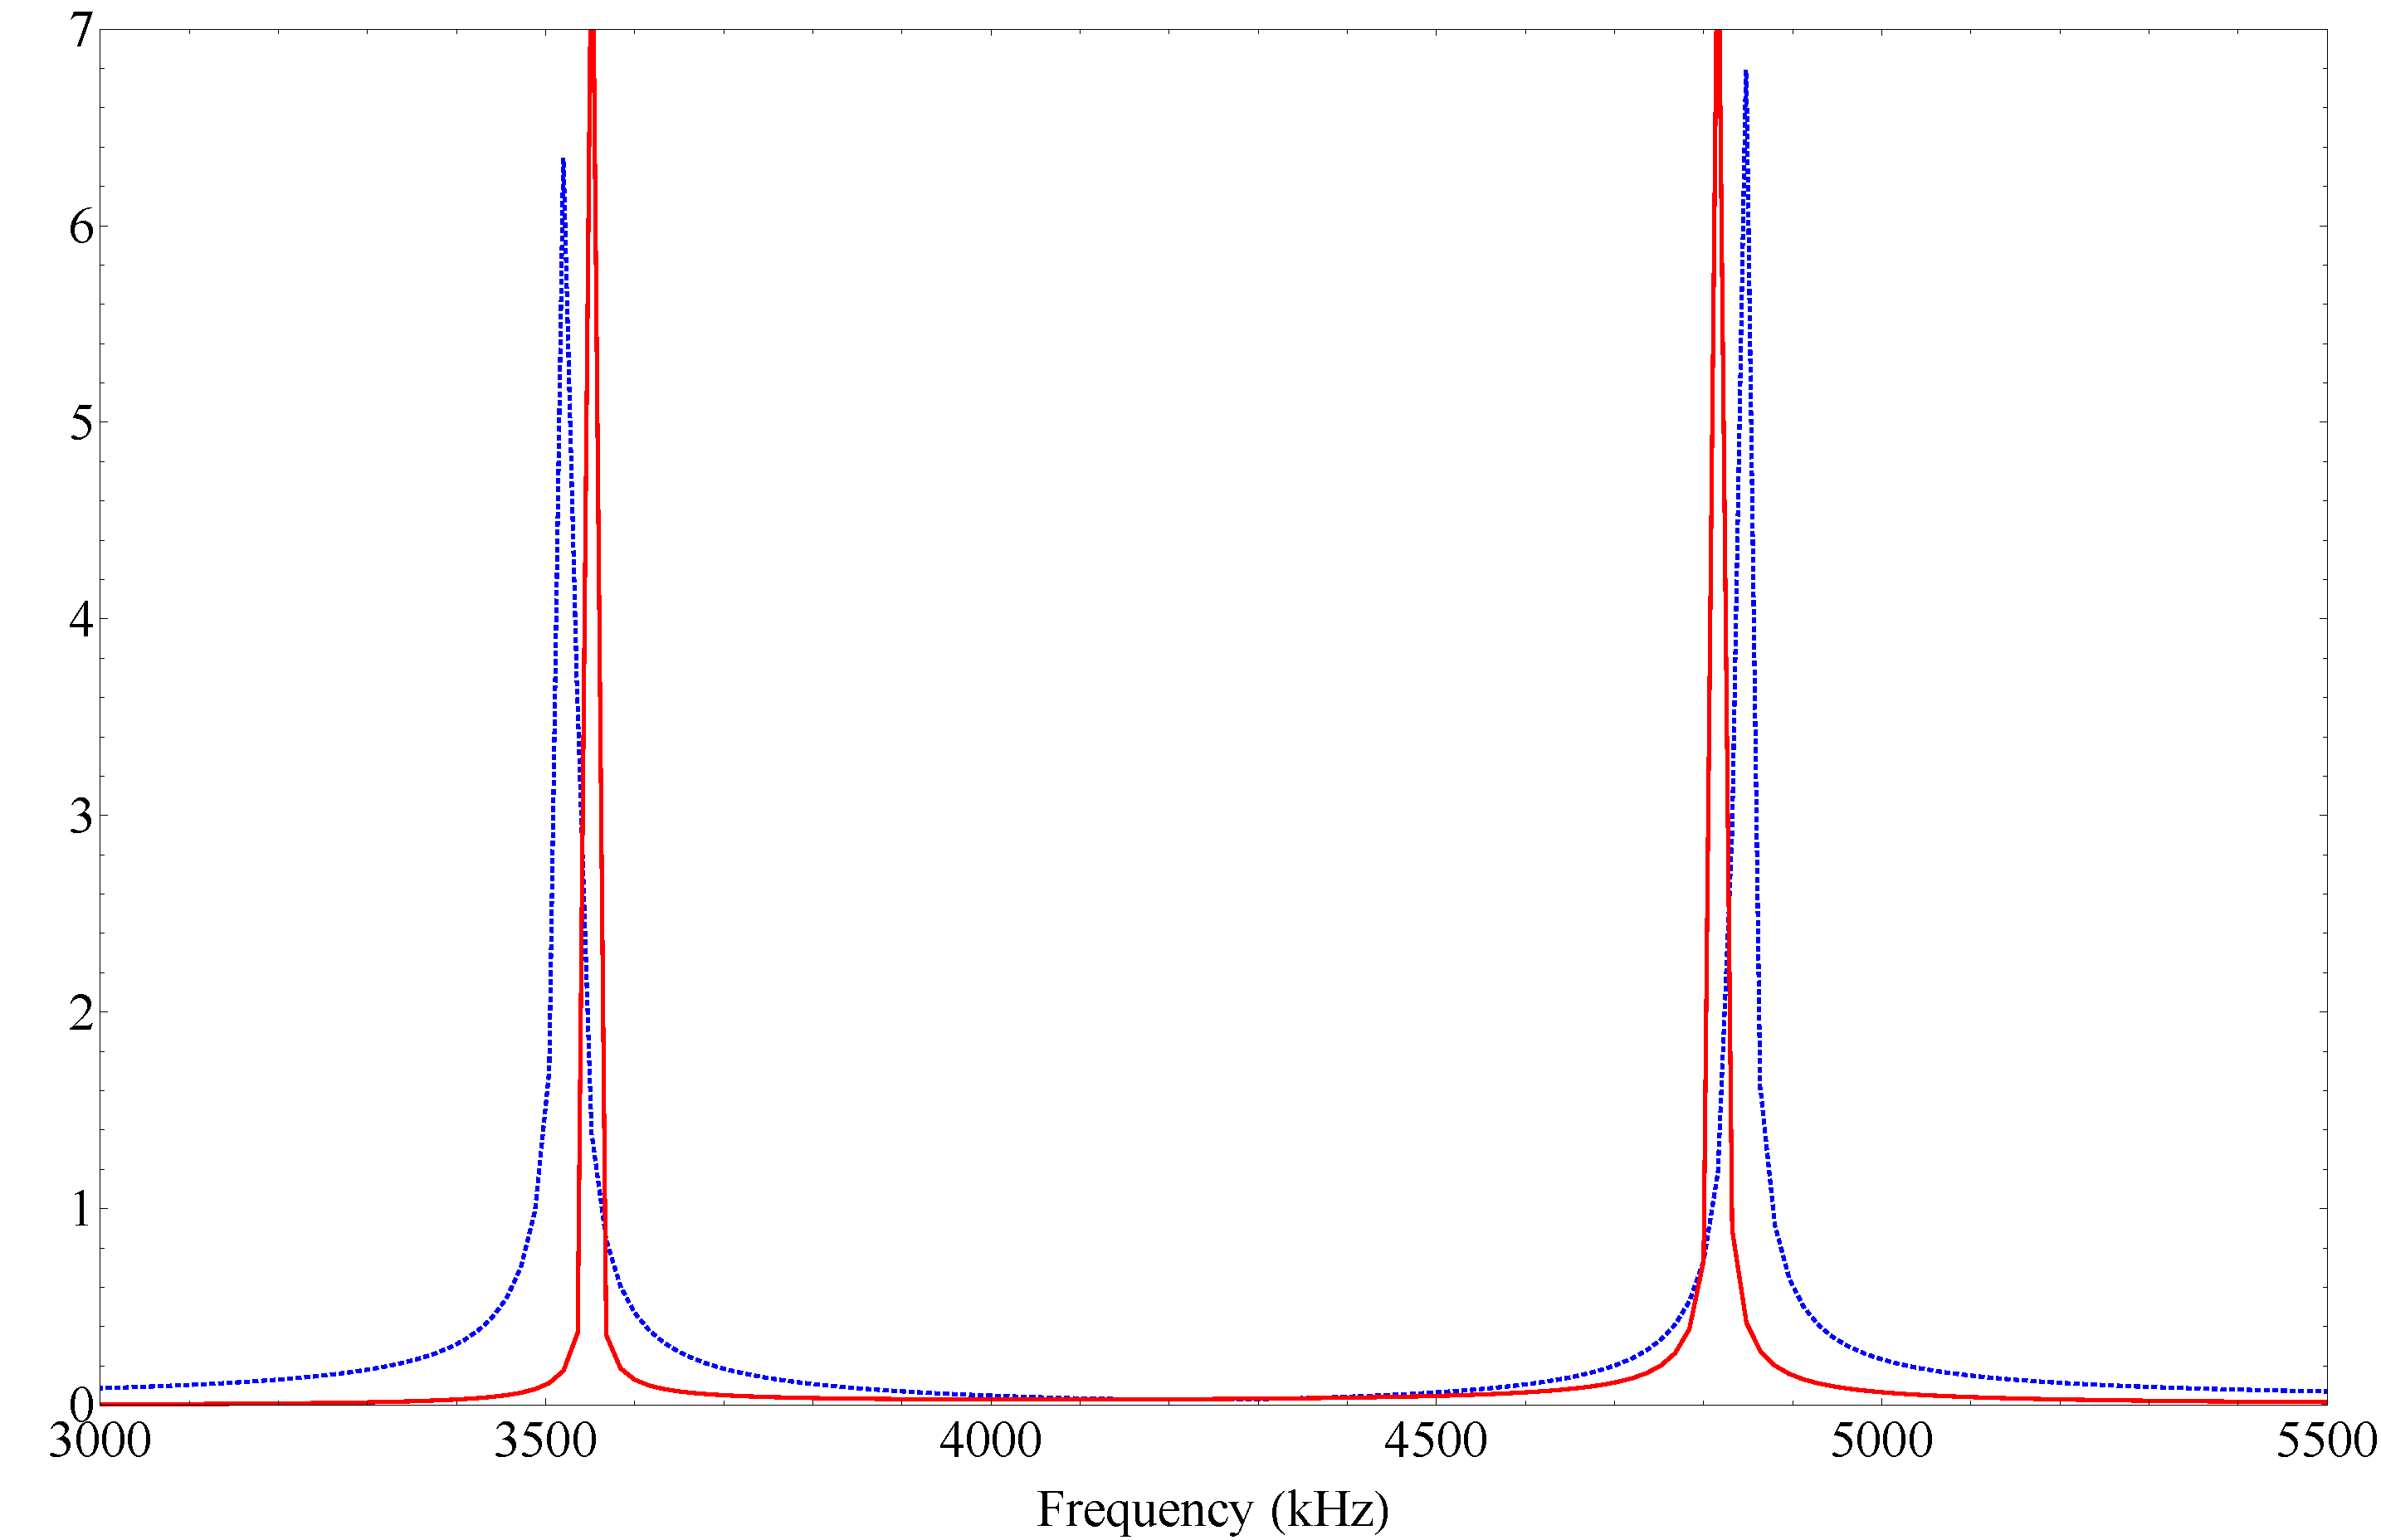
\includegraphics[width=1\columnwidth]{FT10hk.pdf}
\caption{The time-discrete fourier transform of Eq.\ (\ref{prob1}) with a momentum transfer of $\pm10 n_r\hbar k$.  The red line show the frequency fingerprint without the HMW phase, while the blue line include the HMW phase. The frequency splitting due to the HMW phase is now much more apparent compared with the $2\hbar k$ scattering simulation.} 
\label{fig:ft10hk}
\end{figure}

%*********************************************************



 
%*********************************************************
\section{Mach-Zehnder Interferometer}
\label{sec:mach}
%*********************************************************
In this section we consider a Mach-Zehnder interferometer arrangement which can be used to detect the optical HMW phase.  The interferomter uses 3 optical gratings which Raman scatter a collimated and velocity selected atomic beam as seen in fig.\ref{fig:mach}.  
%***************************figure**********************
\begin{figure}
\includegraphics[width=1\columnwidth]{MachZehnder.pdf}
\caption{A Mach-Zehnder inteferometer with a laser applied across one of the arms. The Poynting vector $\vec{S}$ contributes to an HMW phase along the upper and lower paths, but not along the middle arm.} 
\label{fig:mach}
\end{figure}
%*********************************************************
Between the first and second optical gratings, we apply a steady state laser.  The concern here is that the component of the atom beam which travels along the laser direction is very small.  If we assume the velocity of the beam is $10^3\,\mathrm{m/s}$, and the recoil velocity is $10^{-2}\,\mathrm{m/s}$, this gives an angle of $\theta=10^{-5}$ radians.  Using a value of $\alpha E^2=3\times 10^{-25}$ J, we find the HMW phase picked up is 
\begin{equation}
\phi_{\mathrm{HMW}} = \hbar^{-1} \oint [\mathbf{B}(\mathbf{r}) \times \mathbf {d}] \cdot d \mathbf r =10^{-4}d
\end{equation}
Where $d$ is the distance traveled.  We see that this produces too small a value to be detected, so we need to change the arrangement up to get rid of the small interaction angle.  To do this we point the laser along the arm of the upper path after the second optical grating as seen in fig.\ref{fig:mach2}. 
%***************************figure**********************
\begin{figure}
\includegraphics[width=1\columnwidth]{MachZehnder2.pdf}
\caption{A Mach-Zehnder inteferometer with a laser applied along one of the path arms.  The laser must be applied at a slight angle so as to not interfere with the middle arm.  In this image, the laser should be thought of as originating out of the interferometer plane, and passing through it at a very slight angle.} 
\label{fig:mach2}
\end{figure}
%*********************************************************
With this new setup, and assuming the same values as before, we are able to obtain an HMW phase equal to 10 times the interaction length.  We have quite a bit of freedom here in choosing the interaction length as the decay rate at this intensity is approximately $20/\,\mathrm{s}$ and with the atoms traveling at $10^3\,\mathrm{m/s}$, they can cover $10$ cm of laser interaction with only having a $0.2\%$ chance of a spontaneous event occurring.  
At $10$cm, this would give an HMW phase of $\pi$ rad, which would clearly be detectable.  Note that here we are assuming that the laser has no angle of inclination to the plane that the 2 paths create.  However, it would be possible to use a very shallow angle which wouldn't lower this value by more than an order of magnitude, leaving us still in a detectable region.

\vspace{5mm}

There are some obstacles that must be considered when working with this sort of arrangement.  The first of which involves the classical forces felt by the atom upon entering and exiting the laser.  The Lorentz force acting on an atom in the i'th direction is
\begin{equation}
\mathbf{f}_i= \alpha\mathbf{E}\cdot\frac{\partial}{\partial x_i}\mathbf{E}+\alpha\frac{\partial}{\partial t}\left(\mathbf{E}\times\mathbf{B}\right)_i
\label{lorentz4}
\end{equation}
A proposed solution to this is to configure the interferomter so that a second retro reflected laser acts on the middle path at the same time.  This would cancel out the dipole force and also balance out the dipole energy $\frac{1}{2}\alpha E^2$ experienced by the atoms inside the laser.  
The doppler shifted dipole term doesn't affect us here since the velocity of the atom beam is the same in both arms and hence contributes equally.  The only term that now makes an appearance is the Abraham force term $\mathbf{f}_{2i}= \alpha\frac{\partial}{\partial t}\left(\mathbf{E}\times\mathbf{B}\right)_i$.  Let us better understand how the Abraham term will affect the phase of the atoms.  The Abraham terms contributes by increasing/decreasing the kinetic energy of the atom while it's inside the beam.
\begin{eqnarray}
&&\mathrm{\frac{(mv_0+ \Delta P)^2}{2m}=\frac{(mv_0+\alpha\mathbf{E}\times\mathbf{B})^2}{2m}} \nonumber \\
&&\mathrm{=\frac{1}{2}mv_0^2+v_0(\alpha\mathbf{E}\times\mathbf{B}) +H.O.}
\end{eqnarray}
Here $v_0$ is the initial velocity of the atom beam before entering the beam.  We have made use of Hinds and Barnett's result \cite{hinds} that the impulse an atom picks up due to this term upon entering a red detuned laser is $\alpha\mathbf{E}\times\mathbf{B}$. The Lagrangian of the atom upon entering the laser is then given by
\begin{eqnarray}
&&\mathrm{L}=\frac{1}{2}\mathrm{M}\mathbf{v}^2 + \frac{1}{2}\alpha\left(\mathbf{E} +\mathbf{v}\times\mathbf{B}\right)^2 \nonumber \\
&&=\frac{1}{2}\mathrm{M\mathbf{v}^2 - \mathbf{v}\alpha(\mathbf{E}\times\mathbf{B})+\frac{1}{2}\alpha E^2 +H.O.}
\label{lagrangian3}
\end{eqnarray}
Just as we did above, we add in the change in velocity picked up by the atom due to the Abraham term $\Delta(mv)=\alpha\mathbf{E}\times\mathbf{B}$ and substitute it into the Lagrangian to give
\begin{equation}
\mathrm{L}=\frac{1}{2}\mathrm{M\mathbf{v}^2 +\frac{1}{2}\alpha E^2 +H.O.}
\label{lagrangian4}
\end{equation}
We see that the change in kinetic energy due to the Abraham force exactly cancels out the HMW phase shift that we wanted to see!  It would appear we are in trouble, but a quick calculation (See the next section for details) tells us that the wave function of the atom upon entering the laser has the form
\begin{equation}
\psi(x,t)=Ae^{\frac{i}{\hbar}((\hbar k_0 \pm\alpha\mathcal{E}_0B_0)x-E_0 t)}
\end{equation}
Therefore, we see that the wave function acquires an HMW phase from entering the laser.  This shift is given by
\begin{equation}
\mathrm{\phi_{HMW}=\int dx\,\frac{\alpha (E\times B)(x)}{\hbar}}
\end{equation}
Using the values we used previously, we find $\phi_{\mathrm{HMW}}=\pi$ rad.  This would be completely observable.  Note that in this calculation we've assumed some fairly high intensities for the interaction laser.  By dropping the intensity back down to values suggested by Ed Hinds still produces a phase shift in the millirad range which is detectable.    

%*********************************************************
\section{From Quantum to Classical}
\label{sec:classical}
%*********************************************************
We now try to understand how the classical results come out of the quantum treatment of the scenario proposed by Hinds and Barnett \cite{hinds}.  They consider an atom interacting with a place wave laser given by

\begin{equation}
\mathbf{E}=\mathcal{E}(\omega t - kz)\cos{\left(\omega t - kz\right)}
\end{equation}

As they show, the momentum gained by the atom once the atom is fully enveloped by a red detuned pulse is

\begin{equation}
\mathbf{p}_{kinetic}=\frac{\alpha\mathcal{E}_0B_0}{2}
\end{equation}

where $\mathcal{E}_0$ and $B_0$ are the electric and magnetic field amplitudes and $\alpha$ is the electric polarizability.  The classical Lagrangian of an electrically neutral, polarizable atom is given by \cite{wilkens94}
\begin{equation}
\mathrm{L}=\frac{1}{2}\mathrm{M}\mathbf{v}^2 + \frac{1}{2}\alpha\left(\mathbf{E} +\mathbf{v}\times\mathbf{B}\right)^2
\label{lagrangian3}
\end{equation}
Here we have dropped terms involving the magnetic dipole.  Note in this Lagrangian we have included the R\"{o}ntgen interaction $\frac{1}{2}\alpha \mathbf{E}\times \mathbf{B}$ Which is due to the extra motional electric field $\mathbf{v}\times\mathbf{B}$ that the atom see's in it's frame of reference. Using this, we wish to calculate the state of the atom once it has entered the beam.  Upon entering, the momentum of the atom changes to 
\begin{equation}
m\mathbf{v}=m\mathbf{v}_0+\frac{\alpha\mathcal{E}_0B_0}{2}
\end{equation}
Hence, once the atom is totally enveloped by the pulse, the Lagrangian is
\begin{equation}
\mathrm{L}=\frac{1}{2}\mathrm{M}\mathbf{v_0}^2 + \frac{1}{2}\alpha E_0^2 - \frac{1}{2}\alpha E_0 B_0 \mathbf{v}_0
\label{lagrangian3}
\end{equation}
Here we have dropped the higher order term involving $\alpha ^2$.  The dynamics of the atom are governed by this Lagrangian, so presumably in inclusion of the R\"{o}ntgen interaction term should give different dynamics over the scenario in which we didn't include the R\"{o}ntgen term.  Let's check this.  Assume now we didn't take into account the motional electric field.  The Lagrangian of the atom would then be
\begin{equation}
\mathrm{L}=\frac{1}{2}\mathrm{M}\mathbf{v}^2 + \frac{1}{2}\alpha E^2
\label{lagrangian4}
\end{equation}
Upon entering the beam, the momentum of the atom changes to 
\begin{equation}
m\mathbf{v}=m\mathbf{v}_0-\frac{\alpha\mathcal{E}_0B_0}{2}
\end{equation}
Note here the sign change in the second term.  This is due to the fact that now the force acting on the atom is no longer of the form
\begin{equation}
\mathbf{f}_i= \alpha\mathbf{E}\cdot\frac{\partial}{\partial x_i}\mathbf{E}+\frac{\partial}{\partial t}\left(\alpha\mathbf{E}\times\mathbf{B}\right)_i
\label{lorentz4}
\end{equation}
The Abraham term $\frac{\partial}{\partial t}\left(\alpha\mathbf{E}\times\mathbf{B}\right)_i$ is due to the motional electric field and would therefore not be present.  As Hinds and Barnett show, if only the first term in the force (known as the classical dipole force) is present, then the momentum transferred to the atom due to a red detuned pulse is 
\begin{equation}
\mathbf{p}_{kinetic}=-\frac{\alpha\mathcal{E}_0B_0}{2}
\end{equation}
where the minus sign in front appears due to the fact that the impulse due to the Ahbraham term is exactly twice the size as that due to the dipole force term alone, and acting in the opposite direction.  Remarkably we find that the Lagrangian governing the dynamics of the atom inside the pulse in this scenario is also given by
\begin{equation}
\mathrm{L}=\frac{1}{2}\mathrm{M}\mathbf{v_0}^2 + \frac{1}{2}\alpha E_0^2 - \frac{1}{2}\alpha E_0 B_0 \mathbf{v}_0
\label{lagrangian3}
\end{equation}
It appears that both sets of assumptions lead to the same dynamics!  However this isn't the full story.  Let us suppose the initial state of the atom is a plane wave of the form
\begin{equation}
\mathrm{\psi(x_a,t_a)=Ae^{i(kx_a-\frac{E_0 t_a}{\hbar})}}
\end{equation}
Then the wavefunction at some later point in time $(x_b,t_b)$ is given by
\begin{equation}
\psi(x_b,t_b)=\psi(x_a,t_a)e^{{\frac{i(S_{cl})}{\hbar}}}
\end{equation}
Where the classical action $S_{cl}$ is given by
\begin{equation}
S=\int L\, dt
\end{equation}
which as we saw previously was the same for both scenarios in which the R\"{o}ntgen term was or was not included.  What is different between the two is the initial wave function   $\psi(x_a,t_a)$.  The initial wave function upon entering the beam is.
\begin{equation}
\psi(x_a,t_a)=Ae^{\frac{i}{\hbar}((\hbar k_0 \pm\frac{\alpha\mathcal{E}_0B_0}{2})x_a-E_0 t_a)}
\end{equation}
Depending on whether we include (plus) or exclude (minus) the R\"{o}ntgen term.  If we then wish to calculate the expectation value for the momentum inside the pulse, we get
\begin{eqnarray}
<\hat{P}>&=&\int\psi^{*}(x_b,t_b)\,\left(-i\hbar\frac{\partial}{\partial x}\right)\,\psi(x_b,t_b)\,dx \nonumber \\
&=&\hbar\int|\psi(x_b,t_b)|^2(k_0\pm\frac{\alpha\mathcal{E}_0B_0}{2})\,dx \nonumber \\
&=& p_0\pm\frac{\alpha\mathcal{E}_0B_0}{2}
\end{eqnarray}
which is what we expect to find.  


\begin{thebibliography}{8}


\bibitem{vigue1}{S. Lepoutre, A. Gauguet, G. Tr\'{e}nec, M. B\"{u}chner, and J. Vigu\'{e}
Phys. Rev. Lett. \textbf{109}, 120404 (2012).}

\bibitem{vigue2}{S. Lepoutre, A. Gauguet, M. B\"{u}chner, and J. Vigu\'{e}, Phys. Rev. Lett. \textbf{111}, 030401 (2013).}

\bibitem{vigue3}{S. Lepoutre, A. Gauguet, M. B\"{u}chner, and J. Vigu\'{e}, Phys. Rev. A \textbf{88}, 043627 (2013).}

\bibitem{vigue4}S. Lepoutre, J. Gillot, A. Gauguet, M. B\"{u}chner, and J. Vigu\'{e}
Phys. Rev. A \textbf{88}, 043628 (2013).

\bibitem{meystre}{P. Meystre, Atom Optics (Springer-Verlag, New York, 2001).}

\bibitem{pritchard}{S. Gupta, A. E. Leanhardt, A. D. Cronin, and D. E. Pritchard,
C.R. Acad. Sci. IV-Phys. 2, 479 (2001).}

\bibitem{mckellar93}{X. G. He and B. H. J. McKellar, Phys. Rev. A \textbf{47} 3424 (1993).}

\bibitem{wilkens94}{M. Wilkens, Phys. Rev. Lett. \textbf{72}, 5 (1994).}

\bibitem{dowling99}{J. P. Dowling, C. P. Williams, and J. D. Franson
Phys. Rev. Lett. \textbf{83}, 2486 (1999).}

\bibitem{aharanov59}{Y. Aharanov and D. Bohm, Phys. Rev. \textbf{115}, 485 (1959).}

\bibitem{steck}{Daniel A. Steck, "Rubidium 87 D line Data", 2001}

\bibitem{aharanov84}{Y. Aharanov and A. Casher, Phys. Rev. Lett. \textbf{53}, 319 (1984).}

\bibitem{wei95}{H. Wei, R. Han, and X. Wei, Phys. Rev. Lett. \textbf{75}, 2071 (1995).}

\bibitem{chambers60}{R. Chambers, Phys. Rev. Lett. \textbf{5}, 3 (1960).}

\bibitem{tonomura86}{A. Tonomura, N. Osakabe, T. Masuda, T. Kawasaki, J. Endo, S. Yano and H. Yamada, Phys. Rev. Lett. \textbf{56}, 792 (1986).}

\bibitem{olariu85}{S. Olariu and I. Iovitzu Popescu, Rev. Mod. Phys. \textbf{57}, 339 (1985).}

\bibitem{peshkin89}{M. Peshkin and A. Tonomura, \textit{The Aharanov-Bohm Effect} (Springer-Verlag, New York, 1989).}

\bibitem{cimmino89}{A. Cimmino, G. I. Opat, A. G. Klein, H. Kaiser, S. A. Werner, M. Arif, and R. Clothier, Phys. Rev. Lett. \textbf{63}, 380 (1989).}

\bibitem{sangster93}{K. Sangster, E. A. Hinds, S. M. Barnett, and E. Riis, Phys. Rev. Lett. \textbf{71}, 3641 (1993); K. Sangster, E. A. Hinds, S. M. Barnett, E. Riis, and A. G. Sinclair, Phys. Rev. A \textbf{51}, 1776 (1995).}

\bibitem{zeiske95}{K. Zeiske, G. Zinner, F. Riehle, and J. Helmcke, Appl. Phys. B
\textbf{60}, 205 (1995).}

\bibitem{gorlitz95}{A. G\"{o}rlitz, B. Schuh, and A. Weis, Phys. Rev. A \textbf{51}, R4305 (1995).}

\bibitem{yanagimachi02}{S. Yanagimachi, M. Kajiro, M. Machiya, and A. Morinaga,
Phys. Rev. A 65, 042104 (2002).}

\bibitem{Berry}{M. V. Berry and Pragya Shukla, J. Phys. A \textbf{46}, 422001 (2013).}

\bibitem{Nelson}{D.F. Nelson, Phys. Rev. A 44, 3985 (1991).}

\bibitem{Rikken}{G. L. J. A. Rikken, and B. A. van Tiggerlen, Phys. Rev. Lett. 108, 230402 (2012).}

\bibitem{barnett}{S. M. Barnett, Phys. Rev. Lett. 104, 070401 (2010).}

\bibitem{chiao}{J. C. Garrison and R. Y. Chiao, Phys. Rev. A 70, 053826 (2004).}

\bibitem{mansuripur}{M. Mansuripur and A. R. Zakharian, Phys. Rev. E 79, 026608 (2009).}

\bibitem{ketterle}{G. K. Campbell, A. E. Leanhardt, J. Mun, M. Boyd, E. W. Streed, W. Ketterle, and D. E. Pritchard, Phys. Rev. Lett. 94, 170403 (2005).}

\bibitem{feng}{W. She, J. Yu, and R. Feng, Phys. Rev. Lett. 101, 243601 (2008).}

\bibitem{hinds}{E. Hinds and S. M. Barnett, Phys. Rev. Lett. 102, 050403 (2009).}

\bibitem{loudon}{S. M. Barnett and R. Loudon, Phil. Trans. R. Soc. A,  368 (2011).}

\bibitem{lang73}{R. Lang, M. O. Scully and W. E. Lamb, Phys. Rev. A \textbf{7}, 1788 (1973).}

\bibitem{domokos08}{J. K. Asboth, H. Ritsch, and P. Domokos, Phys. Rev. A \textbf{77}, 063424 (2008).}

\bibitem{griffiths}{David J. Griffiths, \textit{Introduction to Electrodynamics} Third Edition (Prentice Hall, New Jersey, 1999).}

\bibitem{cohentannoudji}{C. Cohen-Tannoudji, J. Dupont-Roc, G. Grynberg, \textit{Atom-Photon Interactions} (Wiley Professional, 1989).}

\bibitem{phillips}{M. F. Andersen, C. Ryu, Pierre Clad\'{e}, Vasant Natarajan, A. Vaziri, K. Helmerson, and W.D. Phillips,Phys. Rev. Lett. \textbf{97}, 170406 (2006).}

\bibitem{boshier}{C. Ryu, K. C. Henderson, and M. Boshier, New J. Phys \textbf{16}, 010346 (2014).}

\bibitem{us}{N. Miladinovic, F. Hasan, N. Chisholm, E. A. Hinds, and D. H. J. O'Dell, Phys. Rev. A \textbf{84}, 043822 (2011).}

\bibitem{preble07}{S. F. Preble, Q. Xu, and M. Lipson, Nat. Photon. \textbf{1}, 293 (2007).}

\bibitem{pfeifer07}{Robert N. C. Pfeifer, Timo A. Nieminen, Norman R. Heckenberg, and Halina Rubinsztein-Dunlop, Rev. Mod. Phys. \textbf{79}(4) 1197-1216 (2007)}

\bibitem{Babson09}{David Babson, Stephen P. Reynolds, Robin Bjorkquist, and David j. Griffiths, American association of physics teachers (2009)}

\bibitem{loudon2}{M. Padgett, S. M. Barnett and R. Loudon, J. Mod. Opt.\textbf{50}, 1555 (2003).}

\bibitem{loudon3}{S. M. Barnett and R. Loudon, J. Phys. B. \textbf{39} ,S671 (2006).}

\bibitem{einstein}{A. Einstein, “The principle of conservation of the centre of gravity movement and the inertia of energy,” Ann. Phys. \textbf{20}, 627–633 (1906).}

\bibitem{Leonhardt2}{Li Zhang, Weilong She, Nan Peng and Ulf Leonhardt, New J. Phys \textbf{17}, 053035 (2015).}

\bibitem{spectroscopy}{R.D. Van Zee, and J.P. Looney, \textit{Cavity-Enhanced Spectroscopy} (Academic Press, 2002).}

\bibitem{cohen-tannoudji-interferometry}{Pippa Storey, Claude Cohen-Tannoudji. The Feynman path integral approach to atomic in-
terferometry. A tutorial. Journal de Physique II, EDP Sciences, 1994, 4 (11), pp.1999-2027.}

\bibitem{Abraham2}{Sharon A. Kennedy, Matthew J. Szabo, Hilary Teslow, James Z. Porterfield, and E. R. I. Abraham, Phys. Rev. A. \textbf{66}, 043801 (2002).}

\bibitem{Allen}{L. Allen, M. W. Beijersbergen, R. J. C. Spreeuw and J.P. Woerdman, Phys. Rev. A. \textbf{45}, 11 (1992).}

\bibitem{Willke}{L. Carbone, C. Bogan, P. Fulda, A. Freise, and B. Willke2, Phys. Rev. Lett. \textbf{110}, 251101 (2013).}

\bibitem{Phillips}{M. F. Andersen, C. Ryu, Pierre Clade, Vsant Natarajan, A. Vaziri, K. Helmerson, and W. D. Phillips, Phys. Rev. Lett. \textbf{97}, 170406 (2006).}

\bibitem{Brevik}{I. Brevik, Phys. Rep. \textbf{52}, 133 (1979).}

\bibitem{pauli}{W. Pauli, Theory of Relativity. New York: Dover, 1981.}

\bibitem{lembessis}{V. E. Lembessis, M. Babiker, C. Baxter, and R. Loudon, Phys. Rev. A. \textbf{48}, 2 (1993)}

\bibitem{padgett}{M. J. Padgett, L. Allen, Optical and quantum electronics, \textbf{31} (1999)}

\bibitem{campbell}{B. Hester, G. K. Campbell, C. LopezMariscal,
C. L. Filguiera, R. Huschka, N. J. Halas and K. Helmerson, Rev. Sci. Instrum. \textbf{83}, 043114}

\bibitem{wilkens2}{M. Wilkens, Phys. Rev. A. \textbf{48}, 6 (1994).}

\bibitem{kasevich}{Chiow S.w., Kovachy T., Chien H.C. and Kasevich M. A., Phys. Rev. Lett., \textbf{107} (2011) 130403.}

\bibitem{courteille}{D. Kruse, C. von Cube, C. Zimmermann, and Ph.W. Courteille, Phys. Rev. Lett., \textbf{91} (2003) 183601.}

\bibitem{hemmerich}{Th. Elsässer, B. Nagorny, and A. Hemmerich, Phys. Rev. A., \textbf{69} (2004) 033403.}


\end{thebibliography}


\end{document}
